\chapter{Konzeption der Anwendung}\label{chapter_3}
Im vorigen Kapitel wurden die Anforderungen, sowie das Umfeld der Arbeit erläutert. In diesem Abschnitt wird der aktuelle Workflow beim Konfigurieren analysiert und anschließend an die mobile Umgebung angepasst. Nach der Workflow-Modellierung wird mit einer Entscheidung über die richtige Plattform fortgefahren.

\section{Aktueller Konfigurationsprozess}
Im aktuellen Prozess des Kunden wird ein Upgrade zuerst über den Produktkatalog gefunden. Im Katalog ist eine eindeutige Nummer enthalten, die bei der Bestellung verwendet wird. Die Fluggesellschaft nennt zu der Upgrade-Nummer, die Flugzeuge, die dieses Upgrade erhalten sollen. Diese Informationen werden von einem Design-Manager angenommen. Für die Weiterverarbeitung werden diese Informationen im Konfigurator-Client aus Abschnitt \ref{airbusConfigurator} erfasst. Die einzelnen Schritte der Erfassung sind in Abbildung \ref{webguiWorkflow} zu sehen. \par
\begin{figure}
\label{webguiWorkflow}
\centering
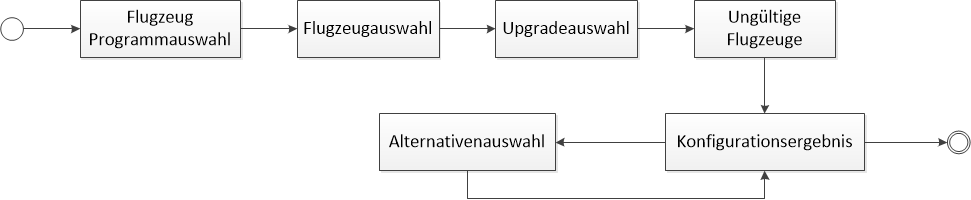
\includegraphics[width=300px]{images/workflow_webgui}
\caption{Programmablauf des Konfigurations-Clients}
\end{figure}
Im ersten Schritt wird das passende Flugzeugprogramm ausgewählt. Ein Programm ist eine grobe Einteilung für Flugzeuge nach deren Größe und Art. Die Auswahl ist eine erste Filterung der Datensätze. Des weiteren wird mit Hilfe des Programms das Regelwerk, welches auf dem Konfigurationsserver verwendet wird festgelegt. Anschließend folgt die Auswahl der entsprechenden Flugzeuge, welche ein Upgrade erhalten sollen. Die Auswahl kann nach bestimmten Kriterien gefiltert werden. Bei der Bestellung eines Upgrades wird die Flugzeugnummer angegeben, womit eine schnelle Auswahl erfolgen kann. Sind die Flugzeuge ausgewählt, werden Upgrades aus einer Liste selektiert. Es sind alle verfügbaren Updates aufgelistet. Die Auswahl erfolgt ebenfalls mit der eindeutigen Nummer, welche bei der Bestellung angegeben wurde. \par 

Nach der letzten Auswahl sind alle für die Konfiguration benötigten Elemente ausgewählt. Es folgt eine Validierung der Flugzeuge. Bei dieser Überprüfung werden die einzelnen Flugzeuge auf Konfigurationen untersucht, die in Widerspruch mit dem ausgewählten Upgrade stehen. Wenn keine Widersprüche gefunden wurden, ist die Bildung von sogenannten Konfigurationsgruppen die nächste Aufgabe. Eine Konfigurationsgruppe enthält Flugzeuge, die in die gleichen Zielzustände kommen, wenn das Upgrade eingebaut wird. Wenn es mehrere Möglichkeiten gibt, um in einen bestimmten Zustand des Flugzeuges zu kommen, werden sogenannte Alternativen in einer Konfigurationsgruppe enthalten. Damit die Konfiguration vollständig ist, muss der Anwender für die Gruppe eine Alternative auswählen. \par

Nachdem eine vollständige Konfiguration erzeugt wurde, wird daraus ein Excel-Dokument generiert. In diesem sind die Upgrades enthalten, die in den einzelnen Flugzeuge eingebaut werden müssen. Aus dem Dokument wird ein Upgrade-Angebot erstellt, dass anschließend dem Kunden vorgelegt wird.

\section{Workflow Modellierung}
Beim derzeitigen Konfigurationsprozess wird die eigentliche Konfiguration dem Experten überlassen. Ein Kunde wählt die Codes und Identifikationsnummern aus Katalog und derzeitigem Flugzeugbestand aus, erhält jedoch erst nach der Arbeit des Experten eine Bestätigung über die Gültigkeit der Konfiguration. Ziel sollte es daher sein, diesen Prozess kundenfreundlicher zu gestalten. Dieses Ziel soll durch folgende zwei Maßnahmen erreicht werden: \par

\begin{itemize}
        \item \textbf{Vereinfachung der Auswahl:} Das An- und Abwählen der Flugzeuge, bzw. der Upgrades soll vereinfacht werden. Die Auswahl soll nicht nur durch die Produktcodes, sondern durch verständlichere Weise erfolgen. 
        \item \textbf{Schnelleres Feedback:} Durch eine mobile Lösung soll bereits beim Kunden ein Feedback über die Gültigkeit der Konfiguration vorhanden sein.
\end{itemize}

Mit beiden Maßnahmen wird der Kunde stärker in den Prozess der Konfiguration einbezogen. Durch die mobile Umgebung ist im neuen Workflow die Möglichkeit gegeben, dass ein Vertriebsexperte mit einem Kunden gemeinsam eine Konfiguration erstellt. Durch diesen Prozess können bspw. Alternativen, die Auftreten besser mit dem Kunden geklärt werden. 
 

 Ziel muss es daher sein, die Auswahl der Konfigurationselemente Flugzeug und Upgrade zu vereinfachen, damit der Kunde besser in den Prozess integriert ist. 

\section{Mobile Plattformen}
\subsection{Native Anwendungen}
\subsection{Web Anwendungen}
\subsection{Hybride Anwendungen}
\subsection{Abwägung}
